\documentclass[a4paper,12pt]{report}
\usepackage{mathtext}
\usepackage[T2A]{fontenc}
\usepackage[utf8]{inputenc}
\usepackage[english,russian]{babel}
\usepackage{geometry}
\usepackage{listings}
\usepackage{amsmath}
\geometry{top=2cm}
\usepackage{titlesec}
\usepackage{color}
\usepackage{blindtext}
\usepackage{pgfplots}
\usepackage{filecontents}
\usetikzlibrary{datavisualization}
\usetikzlibrary{datavisualization.formats.functions}
\usepackage{caption}
\DeclareCaptionFont{white}{\color{white}}
\DeclareCaptionFormat{listing}{\colorbox{gray}{\parbox{\textwidth}{#1#2#3}}}
\captionsetup[lstlisting]{format=listing,labelfont=white,textfont=white}

% Для листинга кода:
\lstset{ %
language=Python,                 % выбор языка для подсветки
basicstyle=\small\sffamily, % размер и начертание шрифта для подсветки кода
numbers=left,               % где поставить нумерацию строк (слева\справа)
numberstyle=\tiny,           % размер шрифта для номеров строк
stepnumber=1,                   % размер шага между двумя номерами строк
numbersep=-5pt,                % как далеко отстоят номера строк от подсвечиваемого кода
showspaces=false,
backgroundcolor=\color{white},         
showstringspaces=false,      % показывать или нет пробелы в строках
showtabs=false,             % показывать или нет табуляцию в строках
frame=single,              % рисовать рамку вокруг кода
tabsize=2,                 % размер табуляции по умолчанию равен 2 пробелам
captionpos=t,              % позиция заголовка вверху [t] или внизу [b] 
breaklines=true,           % автоматически переносить строки (да\нет)
breakatwhitespace=false, % переносить строки только если есть пробел
escapeinside={\%*}{*)},   % если нужно добавить комментарии в коде
	    keywordstyle=\color{blue}\ttfamily,
	    stringstyle=\color{red}\ttfamily,
	    commentstyle=\color{green}\ttfamily,
	    morecomment=[l][\color{magenta}]{\#},
	    columns=fullflexible   % если нужно добавить комментарии в коде
}

% Для измененных титулов глав:
\definecolor{gray75}{gray}{0.75} % определяем цвет
\newcommand{\hsp}{\hspace{20pt}} % длина линии в 20pt
% titleformat определяет стиль
\titleformat{\chapter}[hang]{\Huge\bfseries}{\thechapter\hsp\textcolor{gray75}{|}\hsp}{0pt}{\Huge\bfseries}


% Графики
\begin{filecontents}{InsertionRandom.dat}
100 0.000239
200 0.001058
300 0.002395
400 0.004358
500 0.007077
600 0.010025
700 0.014461
800 0.017972
900 0.023591
1000 0.029958
\end{filecontents}

\begin{filecontents}{CombRandom.dat}
100 0.000087
200 0.000208
300 0.000375
400 0.000548
500 0.000724
600 0.000905
700 0.001038
800 0.001244
900 0.001501
1000 0.001673
\end{filecontents}

\begin{filecontents}{QuickRandom.dat}
100 0.000114
200 0.000236
300 0.000374
400 0.000493
500 0.000630
600 0.000722
700 0.000877
800 0.000971
900 0.001093
1000 0.001206
\end{filecontents}

\begin{filecontents}{InsertionSorted.dat}
100 0.000012
200 0.000023
300 0.000035
400 0.000051
500 0.000065
600 0.000079
700 0.000093
800 0.000107
900 0.000123
1000 0.000136
\end{filecontents}

\begin{filecontents}{CombSorted.dat}
100 0.000068
200 0.000156
300 0.000281
400 0.000431
500 0.000570
600 0.000734
700 0.000861
800 0.001043
900 0.001230
1000 0.001370
\end{filecontents}

\begin{filecontents}{QuickSorted.dat}
100 0.000113
200 0.000243
300 0.000380
400 0.000522
500 0.000661
600 0.000803
700 0.000952
800 0.001101
900 0.001260
1000 0.001412
\end{filecontents}

\begin{filecontents}{InsertionInverse.dat}
100 0.000500
200 0.001982
300 0.004499
400 0.008847
500 0.013292
600 0.019778
700 0.027080
800 0.035924
900 0.046084
1000 0.057707
\end{filecontents}

\begin{filecontents}{CombInverse.dat}
100 0.000076
200 0.000174
300 0.000310
400 0.000496
500 0.000621
600 0.000808
700 0.000946
800 0.001153
900 0.001367
1000 0.001556
\end{filecontents}

\begin{filecontents}{QuickInverse.dat}
100 0.000114
200 0.000246
300 0.000388
400 0.000561
500 0.000673
600 0.000828
700 0.000977
800 0.001138
900 0.001294
1000 0.001474
\end{filecontents}

\begin{document}
\begin{titlepage}
	\centering
	{\scshape\LARGE МГТУ им. Н.Э. Баумана \par}
	\vspace{4cm}
	{\scshape\Large Лабораторная работа №3\par}
	\vspace{0.5cm}	
	{\scshape\Large По курсу: "Анализ алгоритмов"\par}
	\vspace{2cm}
	{\huge\bfseries Алгоритмы сортировки массивов\par}
	\vspace{3cm}
	\Large Работу выполнил: Луговой Дмитрий, ИУ7-51Б\par
	\vspace{0.5cm}
	\Large Преподаватель:  Волкова Л.Л.\par

	\vfill
	\large \textit {Москва, 2019} \par
\end{titlepage}

\setcounter{page}{2}

\tableofcontents

\newpage
\chapter*{Введение}
\addcontentsline{toc}{chapter}{Введение}
\hspace{0.6cm} \textbf{Целью} данной лабораторной работы является исследование существующих алгоритмов сортировки массивов и их трудоемкости.\\
Примем следующую модель вычислений:
\begin{enumerate}
\item Трудоемкость базовых операций\\
Операции $+$, $-$, $*$, $/$, $\%$, $=$, $>$, $<$, $\leq$, $\geq$, $==$, $\neq$, $[\space]$, $+=$, $-=$ - имеют стоимость 1.
\item Трудоемкость условного перехода\\
Условный переход имеет стоимость 0, при этом оцениваем расчет условия:
\begin{align*}
& if \ (n \ \% \ 2 \ == \ 1)\\
& \{\\
&  \ \ \ \ // \ Тело \ 1\\
& \}\\
& else \\
& \{\\
& \ \ \ \ // \ Тело \ 2 \\
& \}
\end{align*}
\[ f_{if} = f_{условия} + \begin{cases} f_{тело \ 1},& при\ нечетном\ N\\ f_{тело \ 2},& при\ четном\ N \end{cases}\\ \]


\item Трудоемкость цикла $for$\\

$f_{цикла} = f_{инициализации} + f_{сравнения} + N(f_{тела} + f_{инкремента} + f_{сравнения})$,

где $N$ - число повторений цикла.
\end{enumerate}
\newpage
\textbf{\LARGE Задачи работы}\\\\
Задачами данной лабораторной являются:
\begin{enumerate}
  	\item Реализовать следующие алгоритмы сортировки массивов:
  	\begin{itemize}
		\item Сортировка вставками
		\item Сортировка расческой
		\item Быстрая сортировка
	\end{itemize}
	\item Проанализировать трудоемкость данных алгоритмов
	\item Провести эксперименты с замерами времени
\end{enumerate}


\chapter{Аналитическая часть}
\hspace{0.6cm}В этом разделе содержатся описания алгоритмов сортировки массивов.

\section{Сортировка вставками}
\hspace{0.6cm} \textbf{Сортировка вставками} (англ. Insertion sort) — алгоритм сортировки, в котором элементы входной последовательности просматриваются по одному, и каждый новый поступивший элемент размещается в подходящее место среди ранее упорядоченных элементов.
Cортировка вставками делит массив на 2 части — отсортированную и неотсортированную. Из неотсортированной части извлекается текущий элемент. Поскольку другая часть массива отсортирована, то в ней достаточно быстро можно найти место для этого извлечённого элемента. Элемент вставляется куда нужно, в результате чего отсортированная часть массива увеличивается, а неотсортированная уменьшается.

\section{Сортировка расческой}
\hspace{0.6cm} \textbf{Сортировка расческой} (англ. Comb sort) - это модификация пузырьковой сортировки. Производятся неоднократные прогоны по массиву, при которых сравниваются пары элементов. Если они неотсортированы друг относительно друга - то производится обмен. В результате крупные элементы мигрируют в конец массива, а небольшие по значению - в начало.
В пузырьковой сортировке при каждом прогоне по массиву сравниваются соседние элементы. Здесь же сравниваются элементы, между которыми некоторое фиксированное расстояние. При каждом следующем прохождении расстояние уменьшается, пока не достигнет минимальной величины.
Уменьшающееся расстояние между сравниваемыми элементами рассчитывается с помощью специальной величины, называемой фактором уменьшения. Длина массива делится на этот фактор, это и есть разрыв между индексами. После каждого прохода расстояние делится на фактор уменьшения и таким образом получается новое значение. В конце концов оно сужается до минимального значения - единицы, и массив просто досортировывается обычным "пузырьком".
В результате практических тестов и теоретических исследований оптимальное значение для фактора уменьшения определено следующее: $\frac{1}{1 - \frac{1}{e^{\varphi}}}$
\section{Быстрая сортировка}
\hspace{0.6cm} \textbf{Быстрая сортировка} (англ. Quick sort) — один из самых известных и широко используемых алгоритмов сортировки.Общая идея алгоритма состоит в следующем:
\begin{itemize}
\item Выбрать из массива элемент, называемый опорным. Это может быть любой из элементов массива. От выбора опорного элемента не зависит корректность алгоритма, но в отдельных случаях может сильно зависеть его эффективность.
\item Сравнить все остальные элементы с опорным и переставить их в массиве так, чтобы разбить массив на три непрерывных отрезка, следующих друг за другом: «элементы меньшие опорного», «равные» и «большие».
\item Для отрезков «меньших» и «больших» значений выполнить рекурсивно ту же последовательность операций, если длина отрезка больше единицы.
\end{itemize}

\chapter{Конструкторская часть}
\hspace{0.6cm}В этом разделе содержатся cхемы алгоритмов сортировки массивов и подсчет трудоемкости.
\newpage
\section{Схемы алгоритмов}

\hspace{0.6cm}На Рис.2.1 представлена схема алгоритма сортировки массивов вставками.
\begin{figure}[ht!]
\center{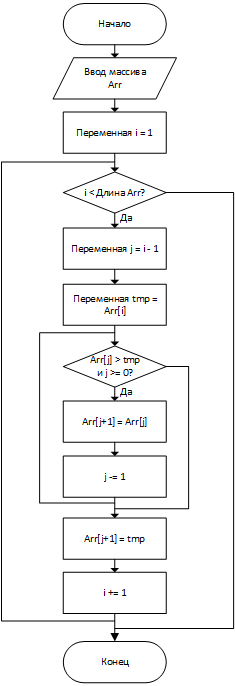
\includegraphics[scale=1]{Insertion.png}}
\caption{Алгоритм сортировки вставками}
\newpage
\end{figure}
\newpage

На Рис.2.2 представлена схема алгоритма сортировки массивов расческой.
\begin{figure}[ht!]
\center{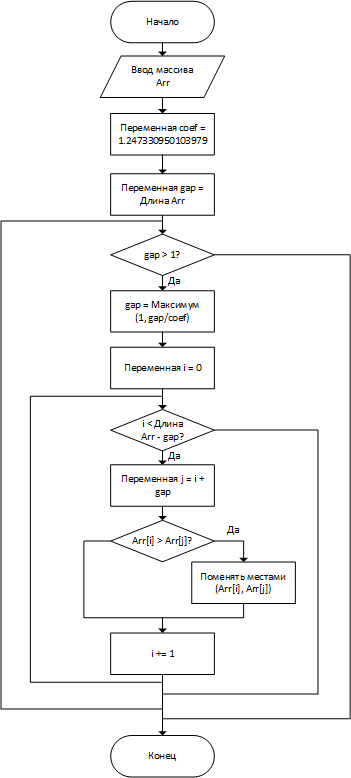
\includegraphics[scale=1]{Comb.png}}
\caption{Алгоритм сортировки расческой}
\end{figure}
\newpage

На Рис.2.3 представлена схема алгоритма быстрой сортировки массивов.

\begin{figure}[ht!]
\center{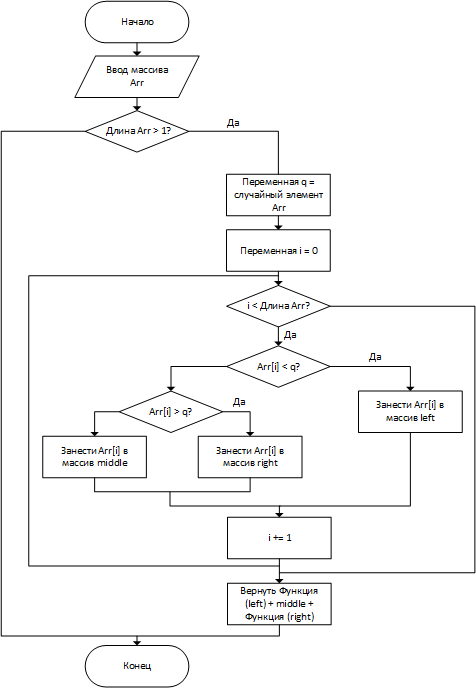
\includegraphics[scale=1]{Quick.png}}
\caption{Алгоритм быстрой сортировки}
\end{figure}
\newpage


\section{Расчет трудоемкости}

\hspace{0.6cm}Пусть задан массив размерности N. Используя модель вычислений, заданную ранее, произведем подсчет трудоемкости алгоритмов сортировки:
\begin{enumerate}
\item \textbf{Сортировка вставками}
\begin{itemize}
\item \textbf{Лучший случай} - отсортированный массив. В этом случае внутренний цикл выполняться не будет:
\[
f_{вставками} = 2 + (N - 1)(2 + 2 + 2 + 2 + 3) = 11N - 9 \approx 11N 
\]
\item \textbf{Худший случай} - обратно отсортированный массив.В этом случае внутренний цикл будет выполняться максимально большое количество раз.

\begin{multline*}
f_{вставками} = 2 + (N - 1)(2 + 2 + 2 + 3) +  \frac{4 + 4 + 1 + (4+4+1)(N - 1)}{2}(N-1)=\\ =4.5N^2 + 4.5N - 7 \approx N^2
\end{multline*}
\end{itemize}

\item \textbf{Сортировка расческой} \cite{tutorials_point}.
\begin{itemize}
\item \textbf{Лучший случай} - полностью отсортированный массив, как и для сортировки пузырьком, модификацией которого она является. В отличие от сортировки пузырьком, данная сортировка отлично справляется с "черепахами" \ -  элементами которые нужно протащить через весь массив, поэтому имеет трудоемкость: $O(n\cdot \log n)$.

\item \textbf{Худший случай} - обратно отсортированный массив, как и для сортировки пузырьком. Трудоемкость: $O(n^{2})$, однако является самой быстрой из квадратичных сортировок.
\end{itemize}

\item \textbf{Быстрая сортировка} \cite{wiki}.
\begin{itemize}
\item \textbf{Лучший случай} - в наиболее сбалансированном варианте при каждой операции разделения массив делится на две одинаковые (плюс-минус один элемент) части, следовательно, максимальная глубина рекурсии, при которой размеры обрабатываемых подмассивов достигнут 1, составит $\log _{2}n$. В результате количество сравнений, совершаемых быстрой сортировкой, было бы равно значению рекурсивного выражения $C_{n}=2\cdot C_{n/2}+n$, что даёт общую сложность алгоритма $O(n\cdot \log n)$.
\newpage
\item \textbf{Худший случай} - в самом несбалансированном варианте каждое разделение даёт два подмассива размерами 1 и $n-1$, то есть при каждом рекурсивном вызове больший массив будет на 1 короче, чем в предыдущий раз. Такое может произойти, если в качестве опорного на каждом этапе будет выбран элемент либо наименьший, либо наибольший из всех обрабатываемых. При простейшем выборе опорного элемента — первого или последнего в массиве, — такой эффект даст уже отсортированный (в прямом или обратном порядке) массив, для среднего или любого другого фиксированного элемента «массив худшего случая» также может быть специально подобран. В этом случае потребуется $n-1$ операций разделения, а общее время работы составит $\sum _{i=0}^{n}(n-i)=O(n^{2})$ операций.
\end{itemize}
\end{enumerate}

Таким образом, в лучшем случае сортировка вставками имеет наименьшую трудоемкость, равную $O(n)$. Однако в худшем случае она сильно проигрывает быстрой сортировке и сортировке расческой из-за коэффициента при $n^{2}$, при этом быстрая сортировка и сортировка расческой имеют приблизительно одинаковую трудоемкость во всех случаях.

\chapter{Технологическая часть}
\hspace{0.6cm}В данном разделе приведены требования к программнму обеспечению, средства реализации и листинги кода
\section{Требования к ПО}

\hspace{0.6cm}На вход поступает массив чисел, на выходе должен возвращаться результат его сортировки.
	

\section{Средства реализации}
\hspace{0.6cm}Для реализации представленных алгоритмов был выбран язык Python. Время работы алгоритмов было замерено с помощью функции perf\_counter() из библиотеки time.

\section{Листинги кода}

\hspace{0.6cm}В Листинге 3.1 показана реализация алгоритма сортировки вставками.

\begin{lstlisting}[caption=Функция сортировки вставками]
  def insertion(arr):
      result = list(arr)
      for i in range(1, len(result)):
          j = i - 1
          key = result[i]
          while result[j] > key and j >= 0:
              result[j + 1] = result[j]
              j -= 1
          result[j + 1] = key
      return result
\end{lstlisting}
\newpage
В Листинге 3.2 показана реализация алгоритма сортировки расческой.
\begin{lstlisting}[caption=Функция сортировки расческой]
  COMB_COEF = 1.247330950103979
  
  def comb(arr):
      result = list(arr)
      gap = len(result)
      while gap > 1:
          gap = max(1, int(gap / COMB_COEF))
          for i in range(len(result) - gap):
              j = i + gap
              if result[i] > result[j]:
                  result[i], result[j] = result[j], result[i]
      return result
\end{lstlisting}

В Листинге 3.3 показана реализация алгоритма быстрой сортировки.
\begin{lstlisting}[caption=Функция быстрой сортировки]
  def quick(arr):
      if len(arr) <= 1:
          return arr
      else:
          q = random.choice(arr)
          left = []
          middle = []
          right = []
          for elem in arr:
              if elem < q:
                  left.append(elem)
              elif elem > q:
                  right.append(elem)
              else:
                  middle.append(elem)
          return quick(left) + middle + quick(right)
\end{lstlisting}



\chapter{Экспериментальная часть}
В данном разделе приведены примеры работы программы, постановка эксперимента и сравнительный анализ алгоритмов на основе экспериментальных данных.
\section{Функциональное естирование}
\hspace{0.6cm}\textbf {Тест 1: Пустой массив}\\
Массив: [ ]\\
Ожидаемый результат: [ ]\\
Сортировка вставками: [ ]\\
Сортировка расческой: [ ]\\
Быстрая сортировка: [ ]\\\\

\textbf {Тест 2: Массив из 1 элемента}\\
Массив: [ 2 ]\\
Ожидаемый результат: [ 2 ]\\
Сортировка вставками: [ 2 ]\\
Сортировка расческой: [ 2 ]\\
Быстрая сортировка: [ 2 ]\\\\

\textbf {Тест 3: Отсортированный массив}\\
Массив: [ 1, 2, 3, 4, 5, 6 ]\\
Ожидаемый результат: [ 1, 2, 3, 4, 5, 6 ]\\
Сортировка вставками: [ 1, 2, 3, 4, 5, 6 ]\\
Сортировка расческой: [ 1, 2, 3, 4, 5, 6 ]\\
Быстрая сортировка: [ 1, 2, 3, 4, 5, 6 ]\\\\

\textbf {Тест 4: Случайный массив}\\
Массив: [ 6, 2, 4, -4, 1]\\
Ожидаемый результат: [ -4, 1, 2, 4, 6 ]\\
Сортировка вставками: [ -4, 1, 2, 4, 6 ]\\
Сортировка расческой: [ -4, 1, 2, 4, 6 ]\\
Быстрая сортировка: [ -4, 1, 2, 4, 6 ]\\\\

\textbf {Тест 5: Обратно отсортированный массив}\\
Массив: [ 6, 5, 4, 3, 2, 1 ]\\
Ожидаемый результат: [ 1, 2, 3, 4, 5, 6 ]\\
Сортировка вставками: [ 1, 2, 3, 4, 5, 6 ]\\
Сортировка расческой: [ 1, 2, 3, 4, 5, 6 ]\\
Быстрая сортировка: [ 1, 2, 3, 4, 5, 6 ]\\\\

Программа успешно прошла все тестовые случаи, все полученные результаты совпали с ожидаемыми.

\section{Сравение алгоритмов по времени}
\hspace{0.6cm}Для экспериментов использовались массивы, размер которых варьируется от 100 до 1000 с шагом 100, при этом рассматривались 3 случая:
\begin{itemize}
\item Массив заполнен случайными числами
\item Массив отсортирован
\item Массив отсортирован в обратном порядке
\end{itemize}
    Количество повторов каждого эксперимента = 100. Результат одного эксперимента рассчитывается как средний из результатов проведенных испытаний с одинаковыми входными данными.
    

\begin{figure}[ht!]
\begin{center}
\begin{tikzpicture}[scale = 1.1]
\begin{axis}[
    	axis lines = left,
    	xlabel = {Размерность массива},
    	ylabel = {Время(секунды)},
	legend pos=north west,
	ymajorgrids=true,
]
\addplot[color=green] table[x index=0, y index=1] {InsertionSorted.dat}; 
\addplot[color=red] table[x index=0, y index=1] {CombSorted.dat};
\addplot[color=blue] table[x index=0, y index=1] {QuickSorted.dat};
\addlegendentry{Вставками}
\addlegendentry{Расческой}
\addlegendentry{Быстрая}
\end{axis}
\end{tikzpicture}
\caption{Алгоритмы сортировки массивов(отсортированных)}
\end{center}
\end{figure}

На Рис. 4.1 видно, что алгоритм сортировки вставками значительно превосходит другие алгоритмы по времени(в $\approx 10$ раз). При этом алгоритм сортировки расческой превосходит алгоритм быстрой сортировки на $\approx 3\%$.

\begin{figure}[ht!]
\begin{center}
\begin{tikzpicture}[scale = 1.1]
\begin{axis}[
    	axis lines = left,
    	xlabel = {Размерность массива},
    	ylabel = {Время(секунды)},
	legend pos=north west,
	ymajorgrids=true,
]
\addplot[color=green] table[x index=0, y index=1] {InsertionRandom.dat}; 
\addplot[color=red] table[x index=0, y index=1] {CombRandom.dat};
\addplot[color=blue] table[x index=0, y index=1] {QuickRandom.dat};
\addlegendentry{Вставками}
\addlegendentry{Расческой}
\addlegendentry{Быстрая}
\end{axis}
\end{tikzpicture}
\caption{Алгоритмы сортировки массивов(случайных)}
\end{center}
\end{figure}

На Рис. 4.2 видно, что алгоритм сортировки вставками в случае сортировки случайного массива потерял свое превосходство и отставание от других алгоритмов растет практически в геометрической прогрессии от размера массива. Отставание алгоритма сортировки расческой от алгоритма быстрой сортировки составляет $\approx 30\%$, однако оно несущественно по сравнению с временем сортировки вставками.

\begin{figure}[ht!]
\begin{center}
\begin{tikzpicture}[scale = 1.1]
\begin{axis}[
    	axis lines = left,
    	xlabel = {Размерность массива},
    	ylabel = {Время(секунды)},
	legend pos=north west,
	ymajorgrids=true,
]
\addplot[color=green] table[x index=0, y index=1] {InsertionInverse.dat}; 
\addplot[color=red] table[x index=0, y index=1] {CombInverse.dat};
\addplot[color=blue] table[x index=0, y index=1] {QuickInverse.dat};
\addlegendentry{Вставками}
\addlegendentry{Расческой}
\addlegendentry{Быстрая}
\end{axis}
\end{tikzpicture}
\caption{Алгоритмы сортировки массивов(обратно отсортированных)}
\end{center}
\end{figure}

\newpage
На Рис. 4.3 видно, что алгоритм сортировки вставками также проигрывает другим алгоритмам и в худшем случае, причем отставание также растет в геометрической прогрессии от размера массива. Алгоритм сортировки расческой отстает от алгоритма быстрой сортировки на $\approx 5\%$, что по сравнению с сортировкой вставками делает их результаты практически идентичными.

\chapter*{Заключение}
\addcontentsline{toc}{chapter}{Заключение}
\hspace{0.6cm}В ходе работы были изучены и реализованы такие алгоритмы сортировки массивов чисел,как алгоритм сортировки вставками, алгоритм сортировки расческой и алгоритм быстрой сортировки. Был проведен сравнительный анализ перечисленных алгоритмов по трудоемкости и экспериментально подтверждено различие во временнoй эффективности. Было показано, что алгоритм сортировки вставками является лучшим выбором, если массив уже отсортирован или практически отсортирован, однако он значительно проигрывает другим алгоритмам в случаях случайного массива и обратно отсортированного массива. В этих случаях алгоритм быстрой сортировки показывает лучшие результаты, но алгоритм сортировки расческой не сильно ему уступает.

\newpage

\addcontentsline{toc}{chapter}{Список литературы}

\renewcommand\bibname{Список литературы}
\begin{thebibliography}{9} 
\bibitem{tutorials_point} TutorialsPoint Comb Sort [Электронный ресурс]. – Режим доступа: URL: https://www.tutorialspoint.com/Comb-Sort. – (Дата обращения: 25.10.2019)
\bibitem{wiki} Wikipedia Быстрая сортировка [Электронный ресурс]. – Режим доступа: URL: https://ru.wikipedia.org/wiki/Быстрая сортировка. – (Дата обращения: 25.10.2019)
\end{thebibliography}

\end{document}